\section{Мета роботи}
Отримання практичних навичок встановлення та
налаштування віртуальних машин.

\section{Хід роботи}
1. Встановлення віртуальної машини з образом та її запуск \textbf{Windows98}. Для неї я виділив \textbf{512МБ ОЗУ} та \textbf{20ГБ} місця на віртуальному диску:
\begin{figure}[h]
    \centering
    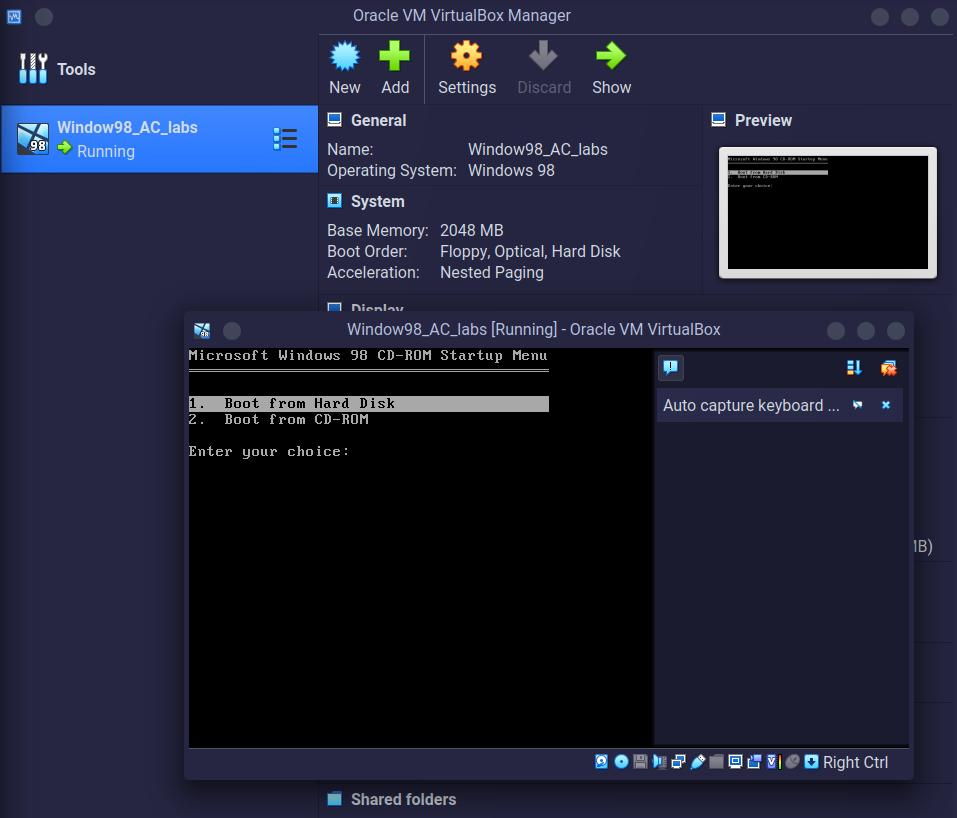
\includegraphics[width=0.8\textwidth]{reports/AC/lab1/assets/1.jpeg}
\end{figure}

\newpage

2. Нижче приведені скріншоти процесу встановки системи:
\begin{figure}[h]
    \centering
    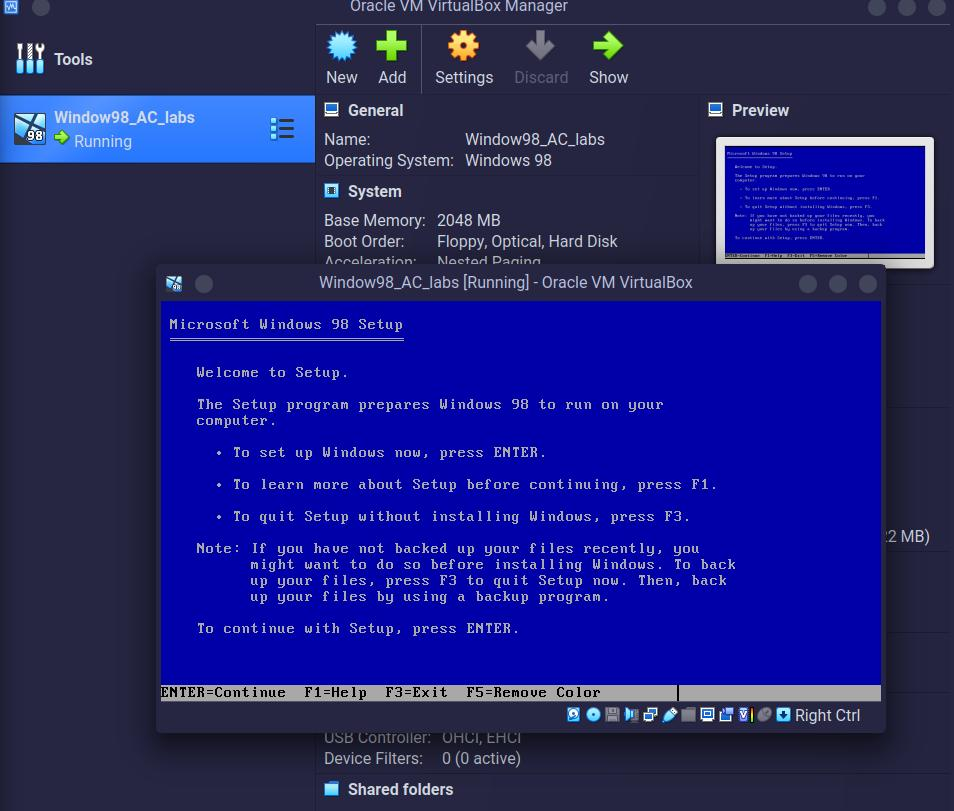
\includegraphics[width=0.6\textwidth]{reports/AC/lab1/assets/2.jpeg}
    \caption{Процес встановки}
\end{figure}

\begin{figure}[h]
    \centering
    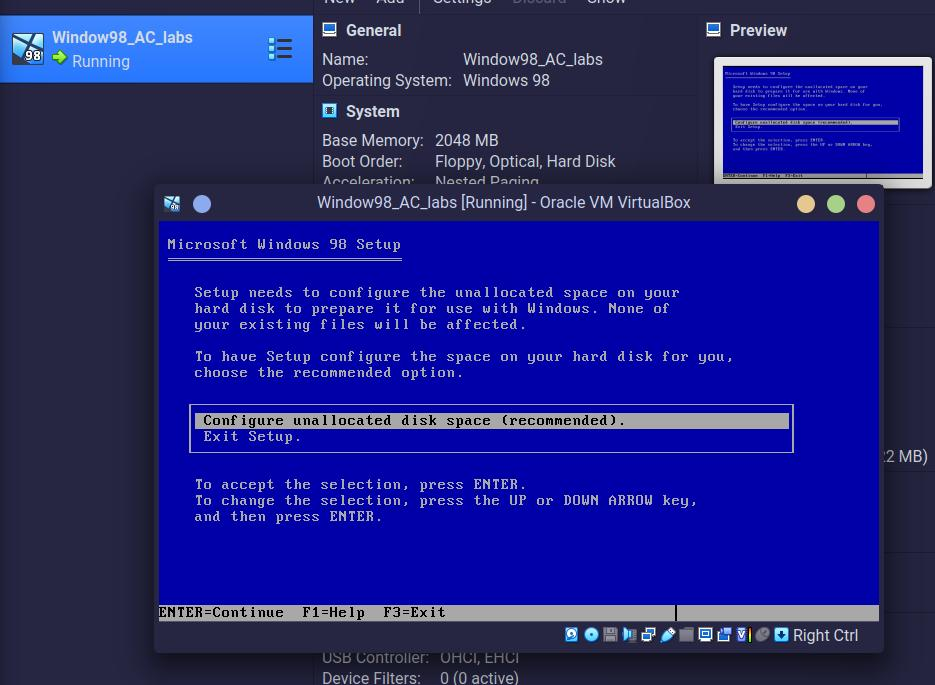
\includegraphics[width=0.6\textwidth]{reports/AC/lab1/assets/3.jpeg}
    \caption{Процес встановки}
\end{figure}

\begin{figure}[h]
    \centering
    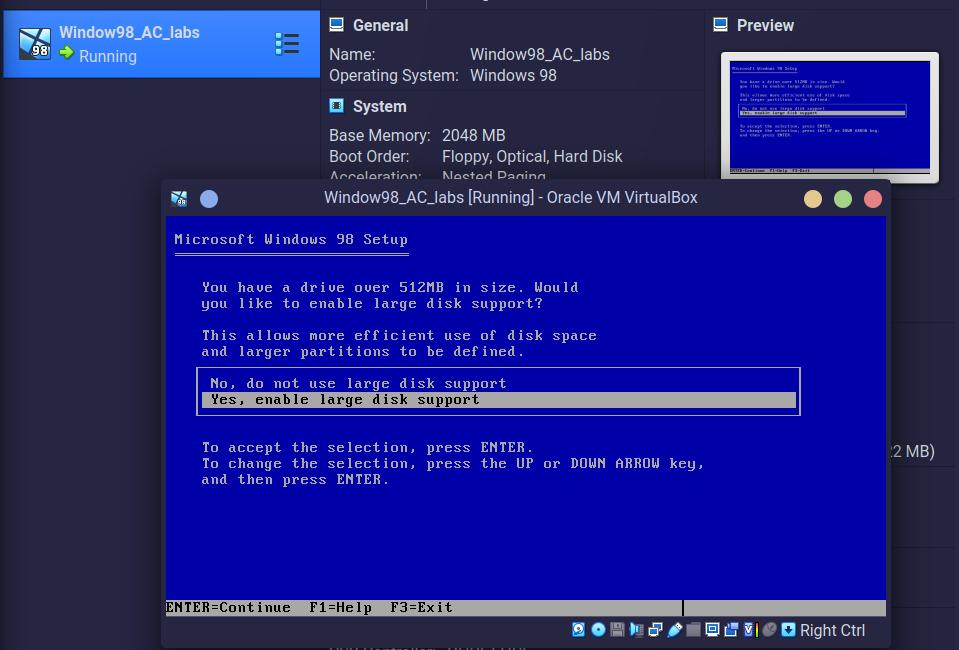
\includegraphics[width=0.7\textwidth]{reports/AC/lab1/assets/4.jpeg}
    \caption{Процес встановки}
\end{figure}

\begin{figure}[h]
    \centering
    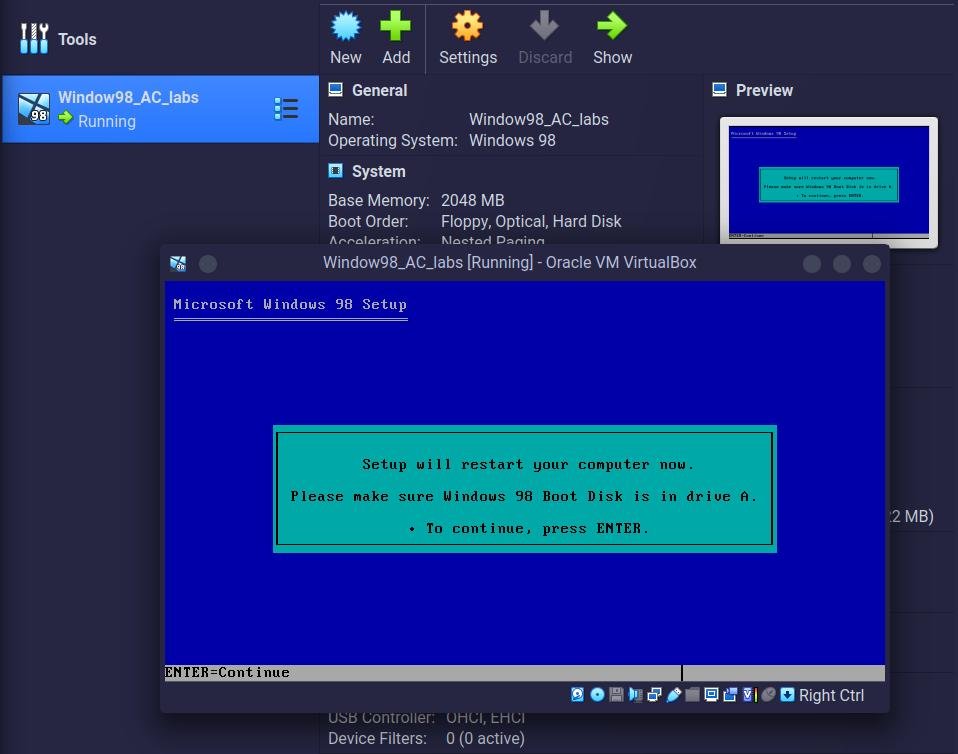
\includegraphics[width=0.7\textwidth]{reports/AC/lab1/assets/5.jpeg}
    \caption{Процес встановки}
\end{figure}

\begin{figure}[h]
    \centering
    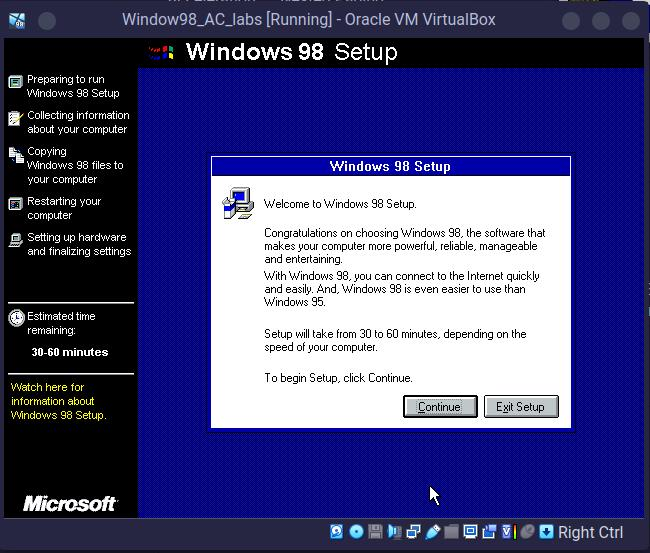
\includegraphics[width=0.7\textwidth]{reports/AC/lab1/assets/6.jpeg}
    \caption{Процес встановки}
\end{figure}

\begin{figure}[h]
    \centering
    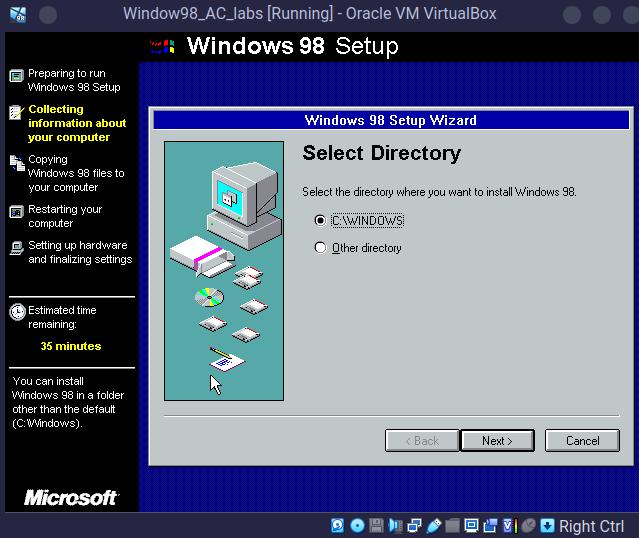
\includegraphics[width=0.7\textwidth]{reports/AC/lab1/assets/7.jpeg}
    \caption{Процес встановки}
\end{figure}

\begin{figure}[h]
    \centering
    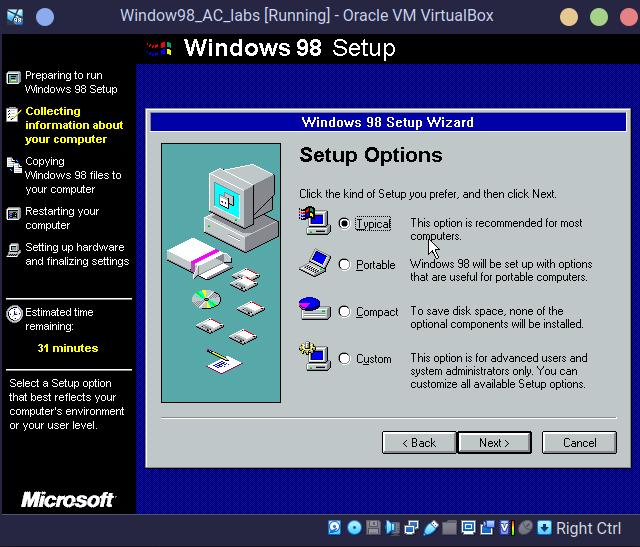
\includegraphics[width=0.7\textwidth]{reports/AC/lab1/assets/8.jpeg}
    \caption{Процес встановки}
\end{figure}

\begin{figure}[h]
    \centering
    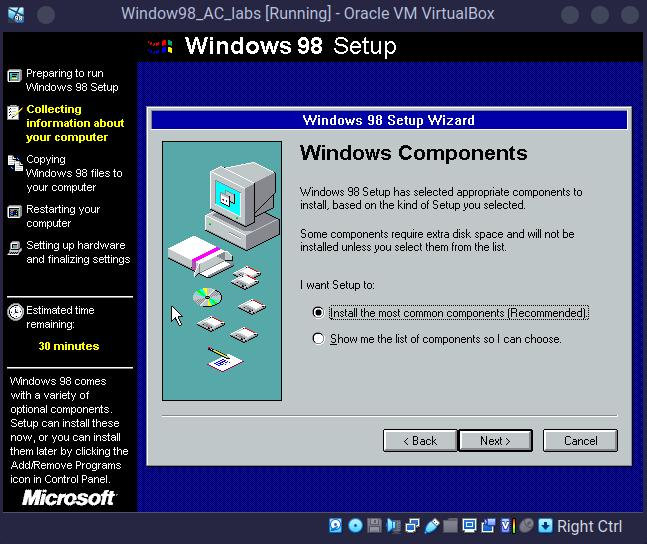
\includegraphics[width=0.7\textwidth]{reports/AC/lab1/assets/9.jpeg}
    \caption{Процес встановки}
\end{figure}

\begin{figure}[h]
    \centering
    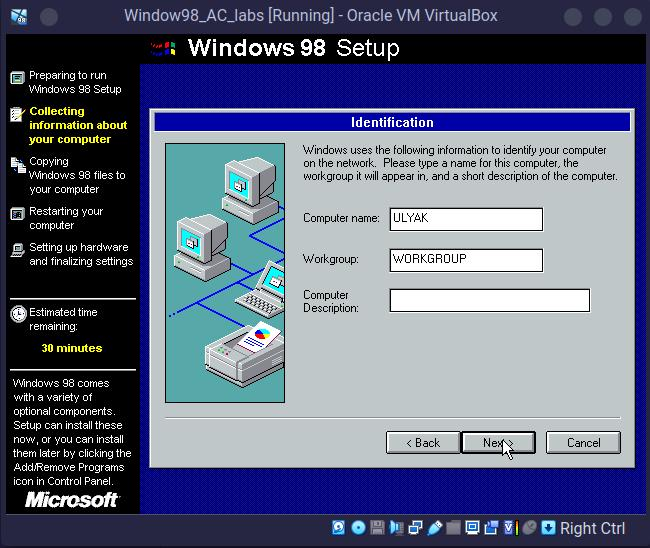
\includegraphics[width=0.7\textwidth]{reports/AC/lab1/assets/10.jpeg}
    \caption{Процес встановки}
\end{figure}

\begin{figure}[h]
    \centering
    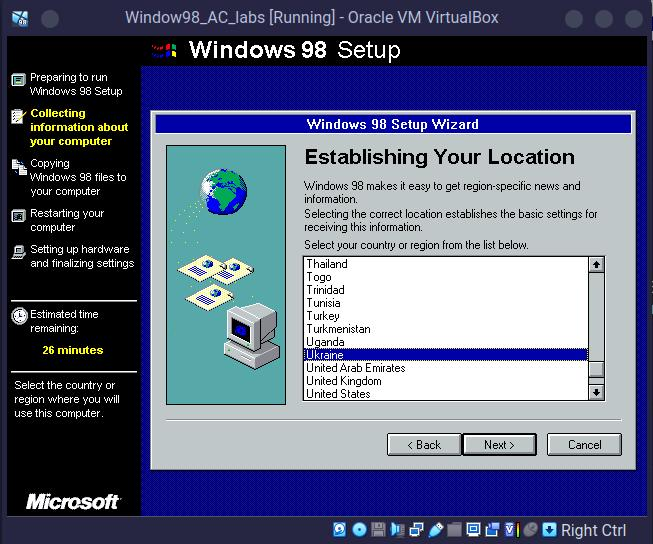
\includegraphics[width=0.7\textwidth]{reports/AC/lab1/assets/11.jpeg}
    \caption{Процес встановки}
\end{figure}

\begin{figure}[h]
    \centering
    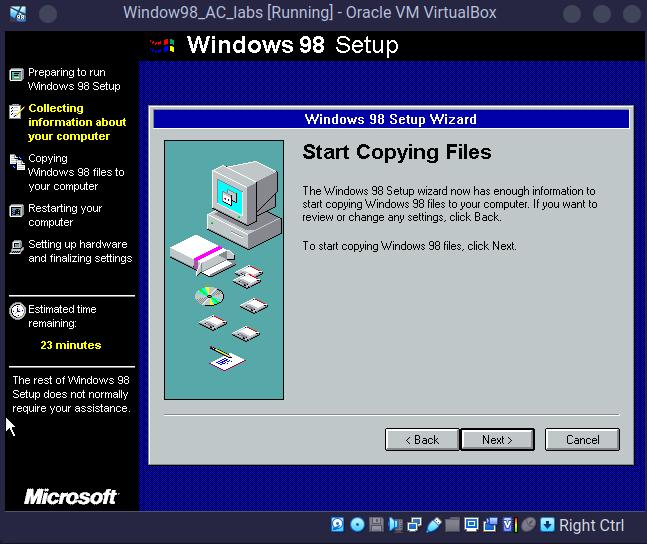
\includegraphics[width=0.7\textwidth]{reports/AC/lab1/assets/12.jpeg}
    \caption{Процес встановки}
\end{figure}

\begin{figure}[h]
    \centering
    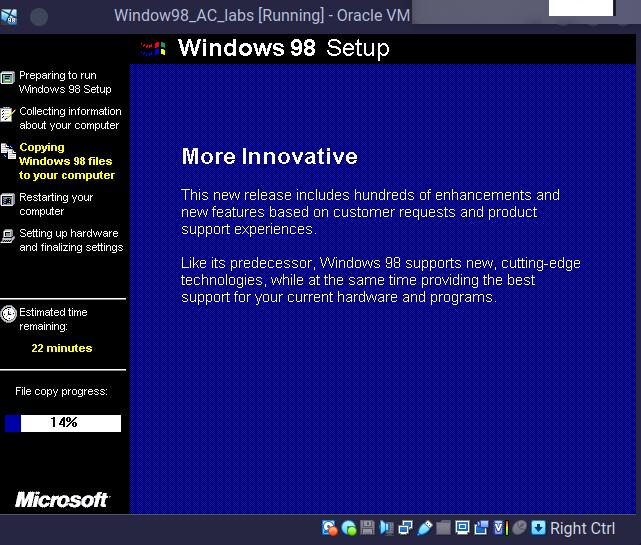
\includegraphics[width=0.7\textwidth]{reports/AC/lab1/assets/14.jpeg}
    \caption{Процес встановки}
\end{figure}

\begin{figure}[h]
    \centering
    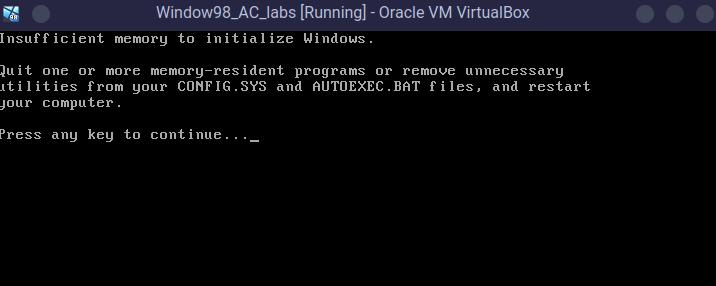
\includegraphics[width=0.7\textwidth]{reports/AC/lab1/assets/15.jpeg}
    \caption{Процес встановки}
\end{figure}

\begin{figure}[h]
    \centering
    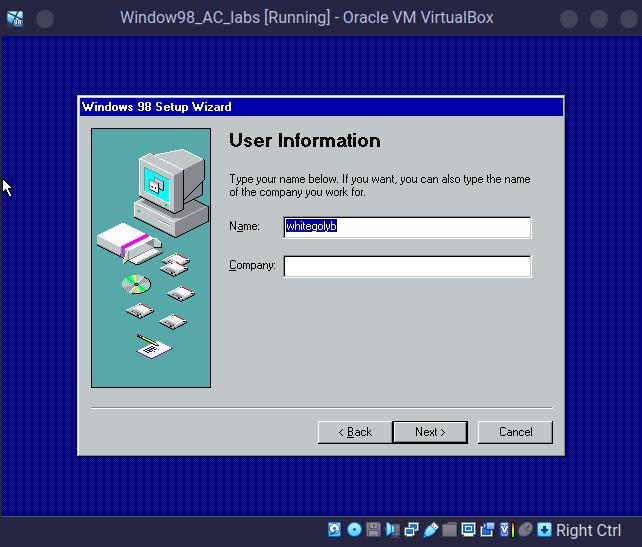
\includegraphics[width=0.7\textwidth]{reports/AC/lab1/assets/16.jpeg}
    \caption{Процес встановки}
\end{figure}

\begin{figure}[h]
    \centering
    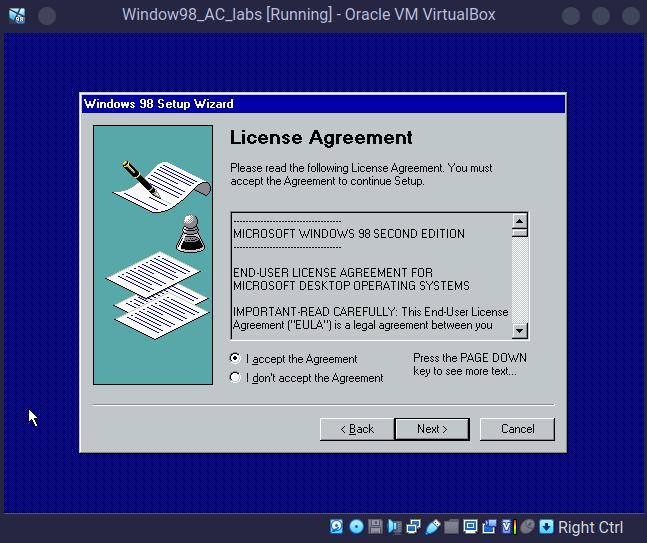
\includegraphics[width=0.7\textwidth]{reports/AC/lab1/assets/17.jpeg}
    \caption{Процес встановки}
\end{figure}

\begin{figure}[h]
    \centering
    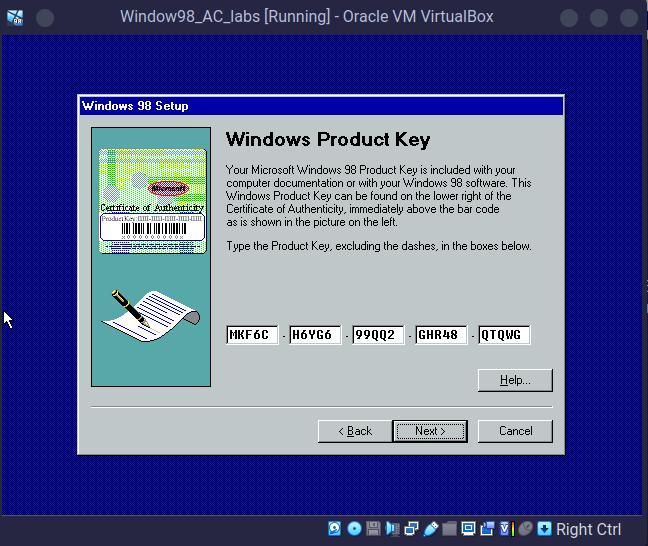
\includegraphics[width=0.7\textwidth]{reports/AC/lab1/assets/18.jpeg}
    \caption{Процес встановки}
\end{figure}

\begin{figure}[h]
    \centering
    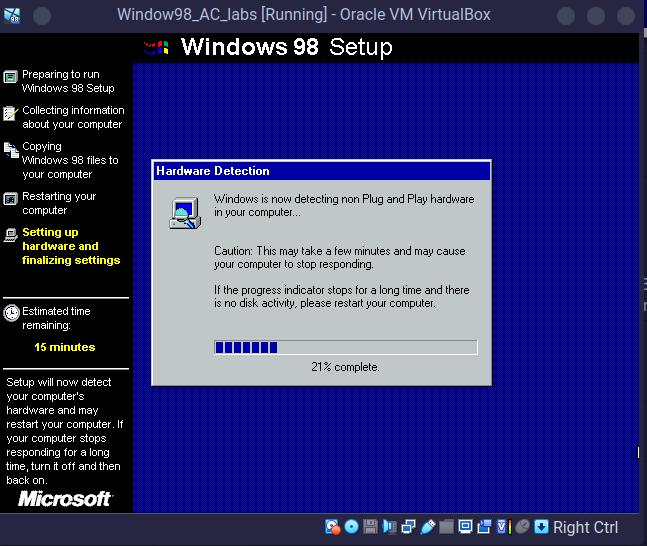
\includegraphics[width=0.7\textwidth]{reports/AC/lab1/assets/19.jpeg}
    \caption{Процес встановки}
\end{figure}

\begin{figure}[h]
    \centering
    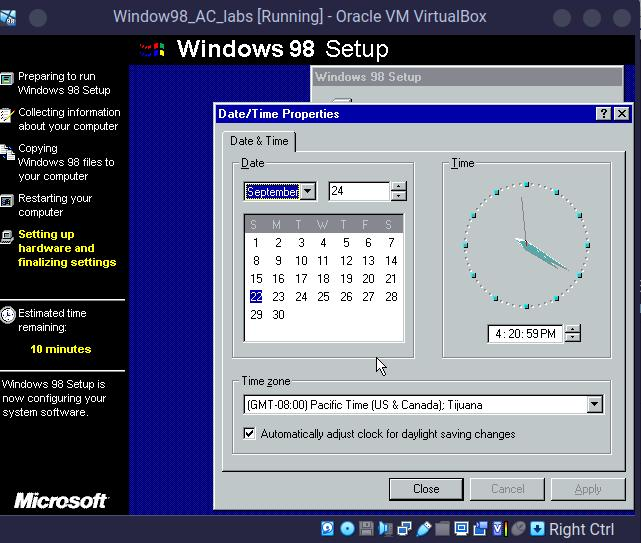
\includegraphics[width=0.7\textwidth]{reports/AC/lab1/assets/20.jpeg}
    \caption{Процес встановки}
\end{figure}

\begin{figure}[h]
    \centering
    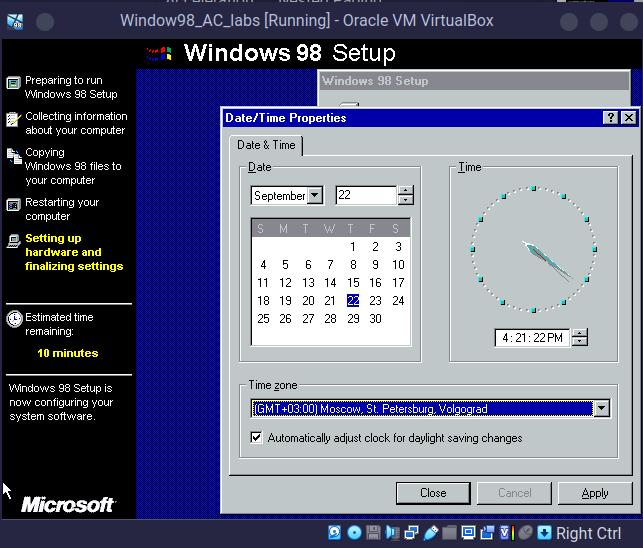
\includegraphics[width=0.7\textwidth]{reports/AC/lab1/assets/21.jpeg}
    \caption{Процес встановки}
\end{figure}

\begin{figure}[h]
    \centering
    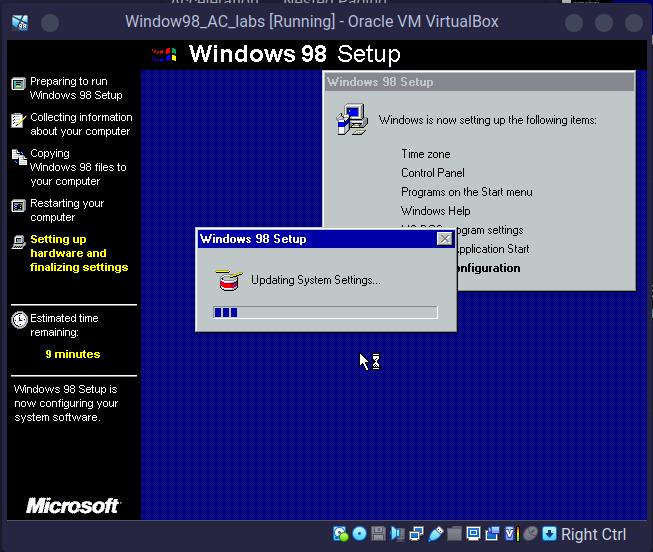
\includegraphics[width=0.7\textwidth]{reports/AC/lab1/assets/22.jpeg}
    \caption{Процес встановки}
\end{figure}

\begin{figure}[h]
    \centering
    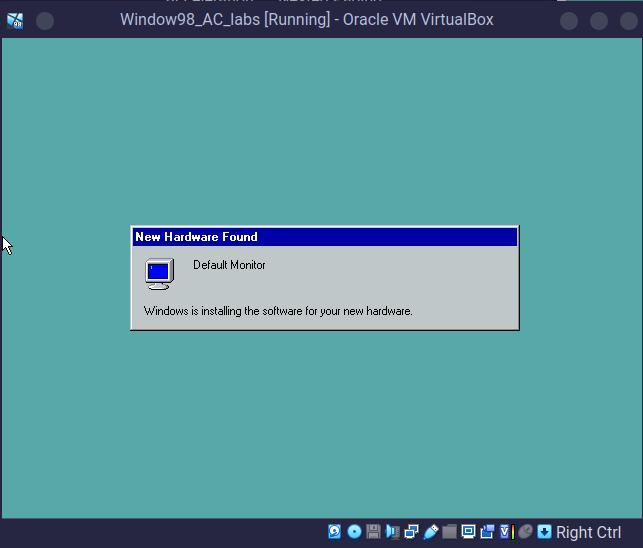
\includegraphics[width=0.7\textwidth]{reports/AC/lab1/assets/23.jpeg}
    \caption{Процес встановки}
\end{figure}

\begin{figure}[h]
    \centering
    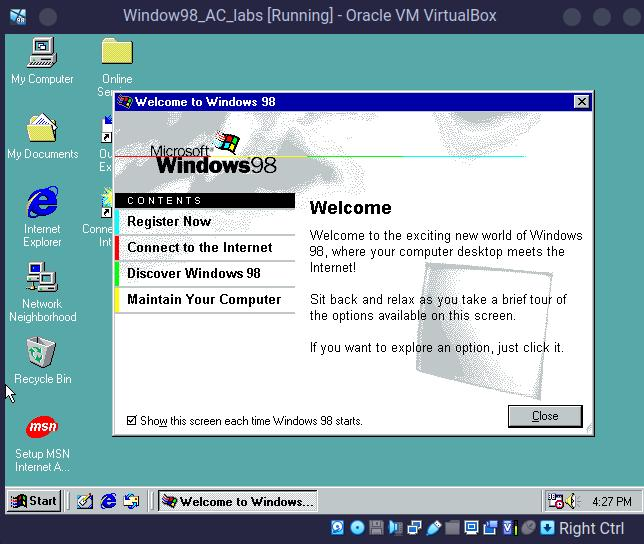
\includegraphics[width=0.7\textwidth]{reports/AC/lab1/assets/24.jpeg}
    \caption{Процес встановки}
\end{figure}


\clearpage
3. Тепер встановлюю \textbf{BorlandC} та роблю базові налаштування для комфортного використання даного інструменту для розробників. Для цього я завантажив та перемістив його у віртуальну машину (обираємо у панелі інструментів запущеної машини \textbf{Devices/Optical Drives/Choose or Create a disk image...}):

\begin{figure}[h]
    \centering
    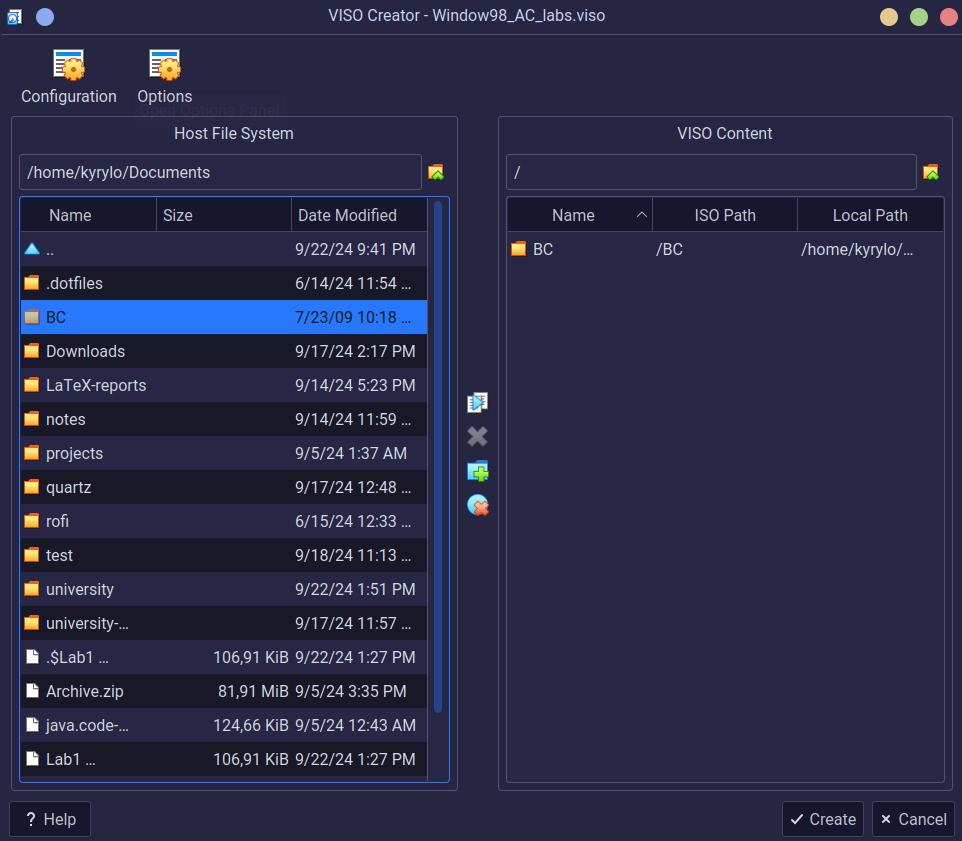
\includegraphics[width=0.5\textwidth]{reports/AC/lab1/assets/26.jpeg}
    \caption{Перенос програми на віртуальну машину}
\end{figure}

4. Переносимо папку з програмою у комфортну директорію та переменую його для комфорту і також додам ярлик на робочий стіл:

\begin{figure}[h]
    \centering
    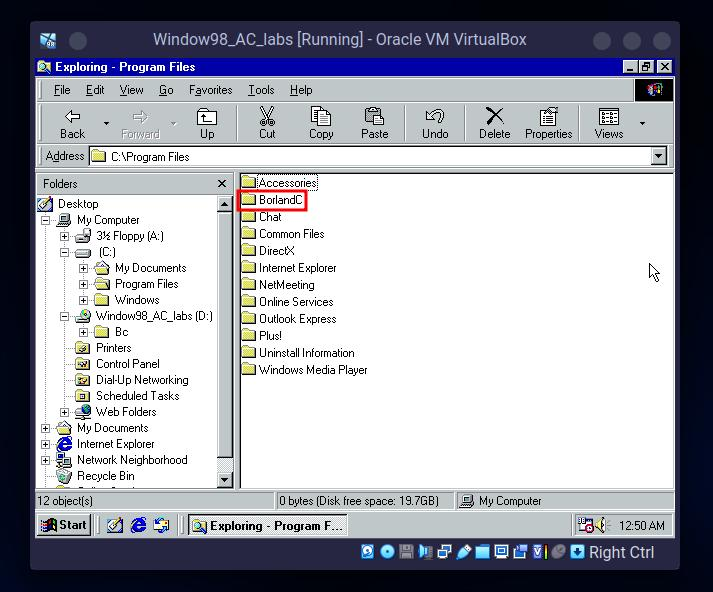
\includegraphics[width=0.6\textwidth]{reports/AC/lab1/assets/28.jpeg}
    \caption{Ярлик для програми}
\end{figure}

\begin{figure}[h]
    \centering
    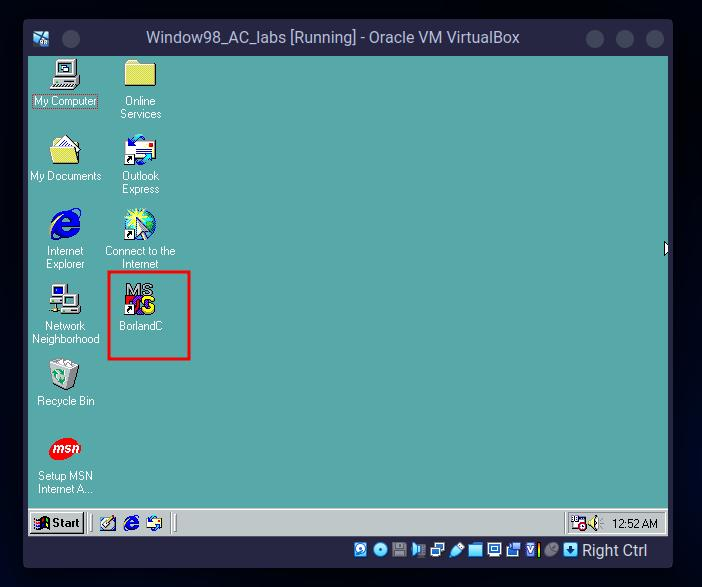
\includegraphics[width=0.9\textwidth]{reports/AC/lab1/assets/29.jpeg}
    \caption{Ярлик для програми}
\end{figure}

\clearpage
5. Також додам програму у змінні оточення, щоб її можна було запустити з будь-якого місця у консолі DOS. Для цього у скрипт автозапуску \texttt{Autoexec.bat} я додав зміни у PATH змінну, і таким чином можна буде запускати програму командою \texttt{bc} у консолі, і це зберігатиметься між сеансами Windows 98:

\begin{figure}[h]
    \centering
    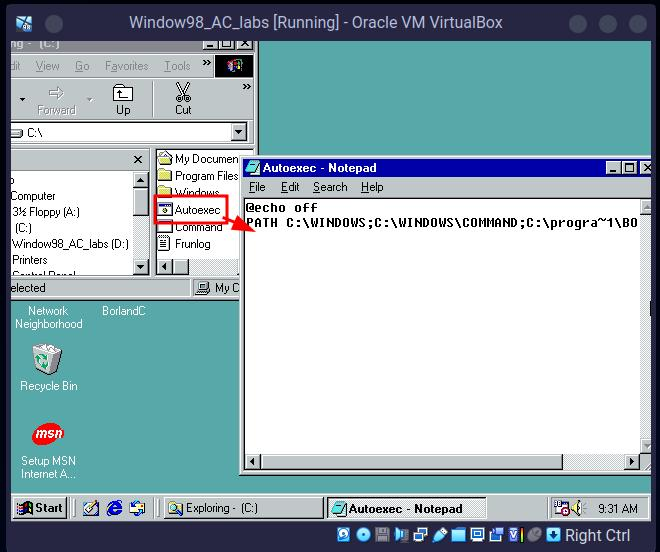
\includegraphics[width=0.7\textwidth]{reports/AC/lab1/assets/30.jpeg}
    \caption{Додаємо зміни у PATH}
\end{figure}

\begin{figure}[h]
    \centering
    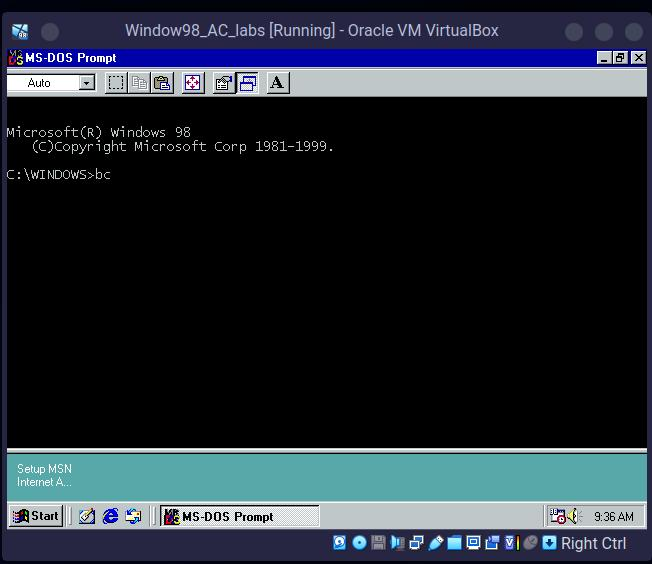
\includegraphics[width=0.7\textwidth]{reports/AC/lab1/assets/31.jpeg}
    \caption{викликаємо за допомогою команди bc}
\end{figure}

\begin{figure}[h]
    \centering
    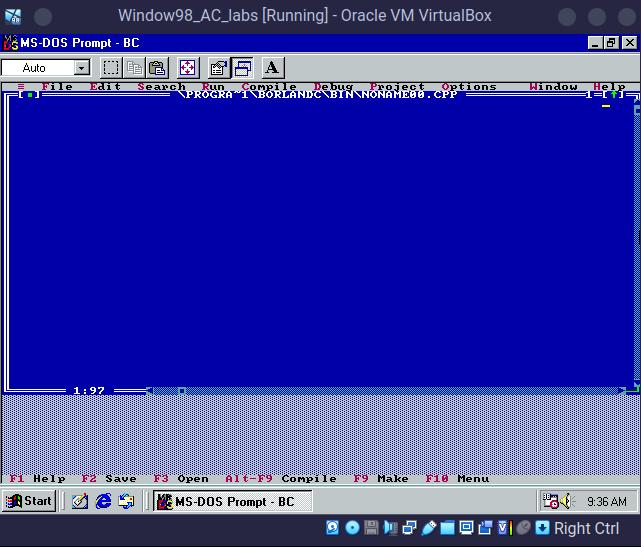
\includegraphics[width=0.7\textwidth]{reports/AC/lab1/assets/32.jpeg}
    \caption{програма відкрилася}
\end{figure}

\clearpage
6. Роблю додаткові налаштування, а саме додаю шляхи до директорій з бібліотеками та компонентами програми і директорії де будуть зберігатися скомпільовані лабораторні роботи:

\begin{figure}[h]
    \centering
    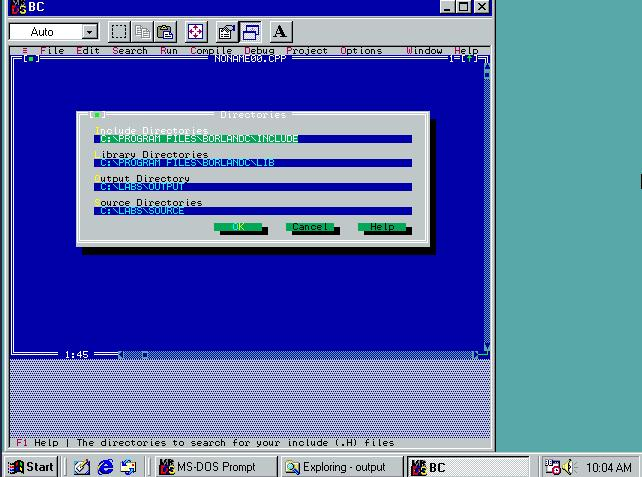
\includegraphics[width=0.9\textwidth]{reports/AC/lab1/assets/33.jpeg}
    \caption{шляхи до важливих директорій}
\end{figure}



\section{Висновки}
Під час виконання лабораторної роботи, я отримав навички по конфігуруванню віртуальнох машини та встановлення на неї Windows98. Працював з графічним та консольним інтерфейсом операційної системи. Успішно встановив у систему програмний пакет BorlandC та налаштував його для подальшого виконання лабораторних робіт.

